% Einleitung
\section{Basics}
\begin{multicols}{2}
\subsection{Euclidean Algorithm}
With the Euclidean Algorithm the $gcd$ is found based on $gcd(a,b)=gcd(b,a \mod b)$.\\ 
Pseudo code:
\begin{verbatim}
int gcd(int a, int b){	=> a>b
  while(b \inq 0){
    r = a mod b
    a = b
    b = r
  }
  return a
}
\end{verbatim}
The \textit{Extended Euclidean Algorithm} returns the $gcd(a,b)$ and calculates $x,y$ $\Rightarrow gcd(a,b)=x a + y b$. 
e.g:\\ 
$gcd(78,99)=3=14 \cdot 78 - 11 \cdot 99$\\
\tr{eucl(a,b)}{$\{x\; y \; gcd(a,b)\}$}\negmedspace; $y=b^{-1} \mod a$\\
\tr{eucl(12,9)}{$\{1\, -\negmedspace 1 \quad 3\}$}$=12-9=3$\\

\subsection{Euler's Phi-Function $\varphi(n)$}
For every natural number $n$, $\varphi(n)$ is the number of natural numbers smaller or equal to $n$ that are coprime (zählerfremd) to $n$.\\
\tr{ephi(n)}{$\varphi(n)$}\\ 

\begin{tabular}{| l l l |}
	\hline
	1:		&	$n=p \to p=\text{prime number(PN)}$				&	$\varphi(n)=p-1$\\
	2:		&	$n=p \cdot q \to p,q=PN$	&	$\varphi(n)=(p-1)(q-1)$\\
	3:		&	$n=p^k \to p=PN$			&	$\varphi(n)=p^k-p^{k-1}$\\
	\hline
\end{tabular}

\subsection{Modular Arithmetic}
If $a \equiv b \mod m$ and $c \equiv d \mod m \to a=b+k \cdot m$; $k \in \mathbb{N}$.
\begin{liste}
\item $a \cdot c \mod m = (a \mod m) \cdot (c \mod m) \Rightarrow$ \\ Reduktion durch kleinere Zahlen
\item $a + b \mod m \equiv b \mod m + d \mod m$
\item $k a \equiv k b \mod m$
\end{liste}%TODO: check properties
\end{multicols}

\subsection{Modular Inverses}
Definition: $a \cdot x \equiv 1 \mod m \Rightarrow x \equiv a^{-1} \mod m$\\
Requirement: $x$ only exists if $gcd(a,m)=1$ ($a$ and $m$ are coprime).\\
Trick: $1 = a \cdot x + m \cdot y \Rightarrow 1 \equiv a \cdot x \mod m$ (use \textit{Extended Euclid (a,m)})\\
BSP: $a = 16, m = 13; a^{-1} \mod m \equiv 5$ \\
\tr{inv(a,m)}{$a^{-1}$}

\subsection{Fermat's Little Theorem}
\begin{tabular}{l  l | l}
	$p$=prime number &	if $a$ and $p$ are coprime ($gcd(a,p)=1$) & if $a$ and $m$ are coprime, where $m>0$\\
	$a^p \equiv a \mod p$ &	$a^{p-1} \equiv 1 \mod p$ & $a^{\varphi(m)} \equiv 1 \mod m$\\
	&&\\
	e.g. $a=3; p=7$ & & e.g. $a$ coprime to $m=15$\\
	$a^2=9\equiv2;a^3\equiv3\cdot2\equiv6;a^4\equiv3\cdot6\equiv4;$ & & $\Rightarrow \varphi(15)=\varphi(3 \cdot 5)=\left(3-1\right)\left(5-1\right)=8$\\
  $a^5\equiv3\cdot4\equiv5; a^6\equiv5\cdot3\equiv1 \mod p$ & $\Rightarrow 3^6 \mod 7 \equiv 1 \mod 7$ & $\Rightarrow a^8 \equiv 1 \mod 15$\\
\end{tabular}\\\\
Note: Fermat's Little Theorem does only give an upper bond for the exponent $e$ such that $a^e=1\mod p$.
For some integers $a$, there may exist an exponent $e<p-1$ such as $a^e \equiv 1 \mod p$.
(e.g. $a=2;p=7 \Rightarrow a^2=4;a^3=8\equiv1 \mod p$)

\subsection{Order of Elements}
$g \in \mathbb{Z}, \quad e \in \mathbb{N}, \quad m \in \mathbb{N} \rightarrow$ smallest possible number $e$ such that \boxed{g^e \equiv 1 \mod m} is called the \textit{order} of $g \mod m$.\\
$g^n \mod m \equiv 1 $ wenn $n=k\cdot e$\\
$g^l = g^k$ if and only if $l\equiv k \mod e$\\ 
$\beta = g^i \mod p \Rightarrow \beta =$ generator modulo $p$ if $gcd(p-1,i)=1$ (coprime)\\
$g$ is called a \textit{generator} $\mod p$, if $\{g^i \mod p : 1 \leq i \leq p-1\}$ coincides with the set $\{1,2,\ldots,p-1\}$.\\
Equivalently: $g$ (\textit{primitive elements}) is a generator modulo $p$, if its order $\mod p$ is $p-1$ (so $e=p-1$).\\
The number of generators $\mod p$ is $\varphi(p-1)$.\\
Examples:
\begin{liste}
	\item $m=13$, computing successive powers of $g=2$, all elements $\mod 2$, except 0: $2^1=2; 2^2=4; 2^3=8; 2^4=16\equiv3; 2^5=6; 2^6=12; 2^7=11; 2^8=9, 2^9=5; 2^{10}=10; 2^{11}=7; 2^{12}=1 \Rightarrow$ element $g=2$ has order $m-1=12$
	\item $p=13; g=2$, $g$ is a generator $\mod p \Rightarrow$ the element $g^i \mod p$ is a generator $\mod p$ exactly if $gcd(i,12)=1$, i.e., $i=1,5,7,11 \Rightarrow$ the generators modulo $13$ are $2,6,7,11$
\end{liste}

\subsection{Chinese Remainder Theorem}
Is a method of solving certain simultaneous systems of congruences.\\
\begin{minipage}{4cm}
$x \equiv a_1 \mod m_1$\\
$x \equiv a_2 \mod m_2$\\
$\ldots$\\
$x \equiv a_n \mod m_n$\\
\end{minipage}
\begin{minipage}{14cm}
$m=\displaystyle\prod_{i=1}^{n} m_i, \quad M_i=m/m_i, \quad gcd(m_i, M_i)=1, 1 \leq i \leq n$\\
$y_iM_i \equiv 1 \mod m_i \to y_i\equiv M_i^{-1} \mod m_i \to$ \tr{eucl($M_i,m_i$)}{$\{.., y_i,.. \}$}, \\
$x=\left(\displaystyle\sum_{i=1}^{n} a_i  y_i M_i \right) \mod m$
\end{minipage}\\
\\
\begin{minipage}{5cm}
Example:\\
$x\equiv a_1 \mod m_1 = 5  \mod 7$\\
$x\equiv a_2 \mod m_2 = 3  \mod 11$\\
$x\equiv a_3 \mod m_3 = 10 \mod 13$\\
$x=?$
\end{minipage}
\begin{minipage}{5cm}
$m=m_1 m_2 m_3 = 7\cdot 11 \cdot 13 = 1001$\\
$M_1=m/m_1=11 \cdot 13 = 143$\\
$M_2=m/m_2=7 \cdot 13 = 91$\\
$M_3=m/m_3=7 \cdot 11 = 77$\\
\end{minipage}
\begin{minipage}{8cm}
With Extended Euclid: (e.g. $y_1=exteucl(M_1,m_1)$)\\
$y_1=5;  y_2=4; y_3=12$; $M_1 y_1 \equiv 1 \mod m_1$\\
$\bm x\equiv a_1\cdot y_1\cdot M_1+a_2\cdot y_2\cdot M_2+a_3\cdot y_3\cdot M_3 (\mod m)$\\
$\bm x\equiv 5\cdot5\cdot143+3\cdot4\cdot91+10\cdot12\cdot77 \equiv \bm{894} \mod 1001$\\
Check $\Rightarrow 894 \mod 7 \equiv 5; \quad 894 \mod 11 \equiv 3;$ etc.
\end{minipage}

\subsection{Faster Exponentiation: Square and Multiply}
To compute moduli efficiently the exponents are divided into powers of $2$ and computed step-for-step:\\
$g^e=g^{\sum_{i=0}^k e_i \cdot 2^i}=\prod_{i=0}^k \left(g^{2^i}\right)^{e_i}=g^{e_0}\cdot\left(g^{e_1}\left(...\left(g^{e_{n-1}}\left(g^{e_n}\right)^2\right)^2...\right)^2\right)^2$
\begin{aufzaehlung}
	\item Write $e$ in binary representation and powers of 2: $e=73=2^0+2^3+2^6$
	\item Compute successively the squares of $g^{2^i} \mod m$: $g=6\Rightarrow$\\ 
		$6^{2^1} \mod 100 = 36;\quad 6^{2^2} \mod 100 \equiv 36^2  \mod 100 \equiv 96;\quad  6^{2^3} \mod 100 \equiv {-4}^2 \mod 100 \equiv 16; \ldots$
	\item Determine $g^e$ as the product of those powers $g^{2^i}$, for which $e_i = 1$: $6^{2^0}\cdot6^{2^3}\cdot6^{2^6}\mod 100\equiv 36 \cdot 16 \cdot -4 \equiv 16\mod 100$
\end{aufzaehlung}
The \textit{Square and Multiply} reduces the computational complexity to $\log_2(e)$ squarings and about $1/2 \log_2(e)$ multiplications.\\
If you reach the limits of the calculator when calculating powers of two, you can divide the power and calculate it in two steps (e.g. $6^{2^{10}}=(6^{32})^{32} \mod 100$).

\subsection{Glossary}%TODO: continue
\begin{minipage}{12.5cm}
\begin{tabular}[]{|l |p{9cm}| }
	\hline
	bijektiv & umkehrbar eindeutig\\
	\hline
	injektiv & Sie besagt, dass jedes Element der Zielmenge $Y$ einmal als Funktionswert angenommen wird.
	Es werden also keine zwei verschiedenen Elemente der Definitionsmenge $X$ auf dasselbe Element in der Zielmenge $Y$ abgebildet.\\
	\hline
	permutation & (Vertauschen) versteht man die Ver\"anderung der Anordnung von Objekten in einer Reihenfolge durch Vertauschen der Elemente.\\
	\hline
	affine Abbildung & lineare Abbildung, es bleibt Kolinearit\"at, Parallelit\"at und Teilerverh\"altnisse erhalten. \\
	\hline
\end{tabular}\\

\end{minipage}
\begin{minipage}{6cm}
\textbf{Irreducible Polynomials in:}\\
\begin{tabular}{l l}
	$GF(2)$				&	$GF(3)$\\
	\hline
	$x$					&	$x^2+1$\\
	$x+1$				&	$x^2+x-1$\\
	$x^2+x+1$			&	$x^2-x-1$\\
	$x^3+x+1$			&	$x^3-x+1$\\
	$x^3+x^2+1$			&	$x^3-x-1$\\
	$x^4+x+1$			&	$x^3+x^2+x-1$\\
	$x^4+x^3+1$			&	$x^3+x^2-x+1$\\
	$x^4+x^3+x^2+x+1$	&	$x^3+x^2-1$\\ 
						&	$x^3-x^2+1$\\ 
						&	$x^3-x^2+x+1$\\ 
						&	$x^3-x^2-x-1$\\ 
\end{tabular}
\end{minipage} \\

\subsection{Polynom division}
\begin{minipage}{10.5cm}
	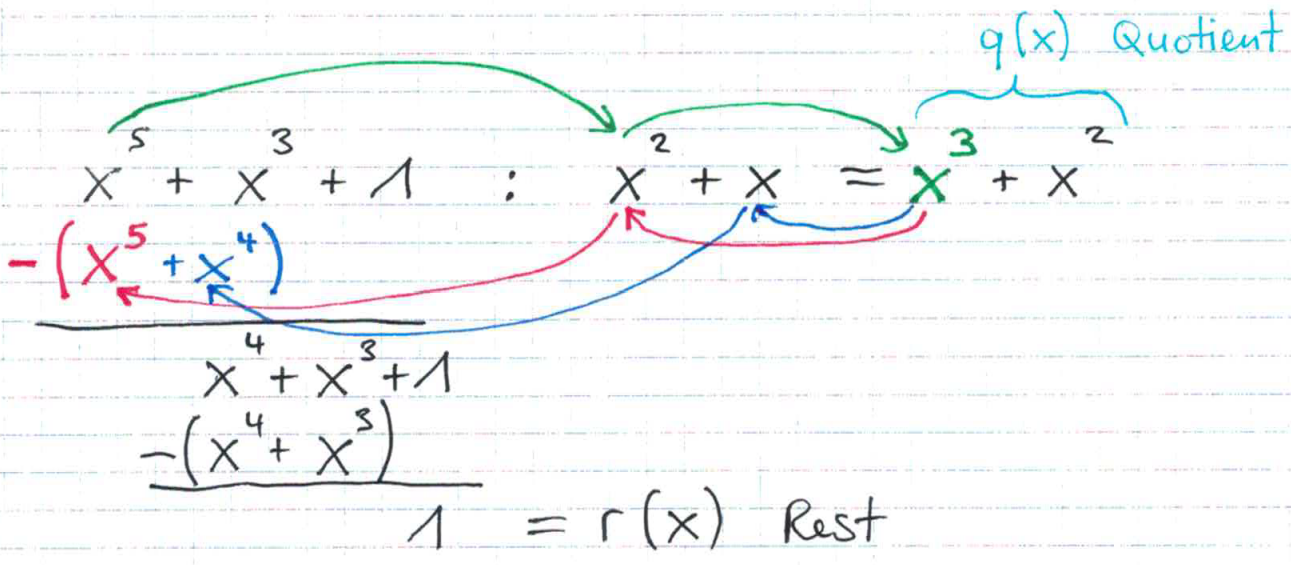
\includegraphics[width=10cm]{./bilder/polynomdivision.png}\\
\end{minipage}
\begin{minipage}{8cm}
	Polynom division can be used to determine whether a given polynomial is irreducible or not, i.e. if the division with any other polynomial (up to the half 
	order of the dividend polynomial) has a rest $r(X)$ or not. In this example, the calculation is done in $GF(2)$, meaning that negative values are 
	equivalent to positive values. In this case $r(X)\neq 0$ and the given polynomial is irreducible.\\
	A polynomial that is not divisible by any polynomial of degree 1 and 2, is also not divisible by any polynomial of higher degree, because a factorization 
	would yield a divisor of degree 1 or 2, respectively.\\
\end{minipage}
